\chapter{Il progetto stage}
\begin{flushright}
	\parbox{13cm}{\small In questo capitolo vengono presentati i due progetti-clienti su cui si è incentrato lo stage.}
\end{flushright}

\section{Primo progetto}
Il primo progetto graficamente rispecchia molto la versione standard del B2B, ma di fatto include varie funzionalità realizzate appositamente per il cliente.
Innanzitutto, essendo questo portale destinato ad agenti e clienti selezionati, per poterlo utilizzare è necessario essere iscritti. L'iscrizione può avvenire in 2 modalità:
\begin{itemize}
	\item l'amministratore crea un account per l'utente, il quale al primo accesso dovrà cambiare password;
	\item l'utente effettua una richiesta di registrazione, che l'amministratore dovrà approvare per rendere attivo l'account. Questa seconda modalità è attivabile tramite il pannello di configurazione dello stesso amministratore.
\end{itemize}
\begin{figure}[H]
	\centering
	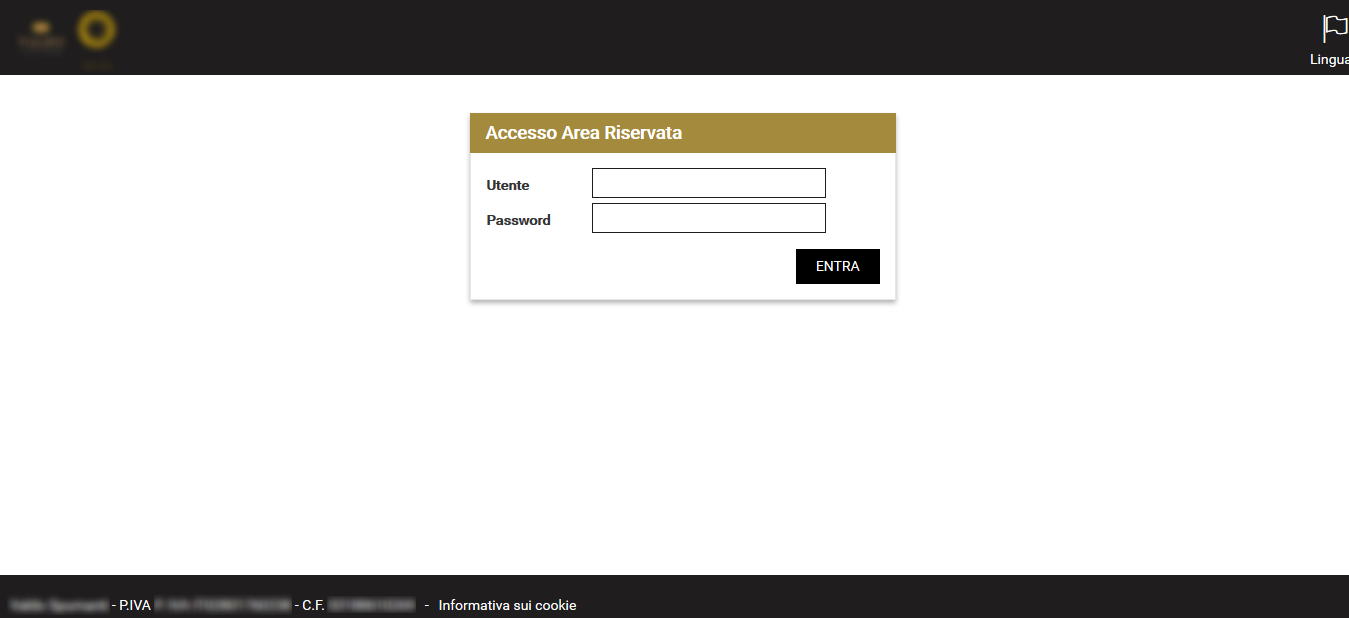
\includegraphics[width=14.5cm]{Immagini/p1/index.png}
	\caption{Pagina di accesso al portale}
\end{figure}

Nel corso delle settimane di stage, sono state svolte alcune implementazioni sulla base di richieste del cliente. Generalmente i lavori svolti per questo progetto erano basati su analisi svolte precedentemente al mio arrivo, in quanto parti dei preventivi presentati al cliente. Prima di iniziare a modificare il codice, mi è tuttavia stato chiesto di presentare in forma di analisi il flusso delle operazioni necessarie per raggiungere l'obiettivo. Le richieste per questo progetto erano legate principalmente all'aggiunta o modifica di informazioni nei risultati o nei parametri di ricerca delle interrogazioni.

Vengono ora presentate alcune delle modifiche effettuate su questo progetto.
\paragraph{Codice cliente}
Il codice cliente è un'informazione chiave nel B2B, in quanto contribuisce ad costruire ed individuare gli ordini. Dal codice cliente dipendono il tipo dell'ordine, i listini, gli sconti e le promozioni. Per questo motivo poter effettuare ricerche tramite questo codice agevola gli agenti e l'amministrazione. Una delle prime richieste è stata proprio di introdurre questa informazione nei parametri e nei risultati delle interrogazioni.
%TODO: inserire screen parametri ricerca
Per agevolare l'utente nell'inserimento di informazioni corrette, è stato predisposto un campo di testo \virgolette{autocompletante}. Una volta digitati tre caratteri nel campo di input viene eseguita una \textit{query} di ricerca nel database per estrarre la lista dei clienti con codice o descrizione (la ragione sociale in termini del gestionale) contenenti la stringa cercata. Questa \textit{query} deve essere il più ottimizzata possibile, in quanto l'utente non deve subire un rallentamento per un'azione come la ricerca, che ha come scopo quello di far raggiungere più rapidamente gli obiettivi. Un approccio alternativo poteva essere quello di caricare la lista di tutti gli utenti nel \textit{backing bean}, per poi utilizzare i metodi offerti dall'interfaccia \texttt{List} per ottenere la sottolista ricercata.

\section{Secondo progetto}
\section{I due progetti a confronto}